\chapter{Planes in Space}

\begin{center}
    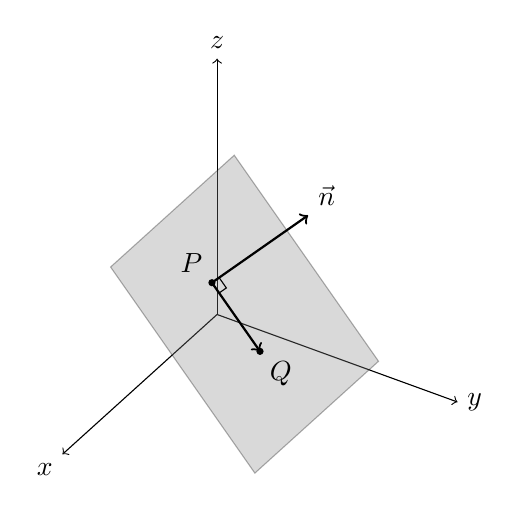
\begin{tikzpicture}[x={({cos(20)},{-sin(20)},0)},z={({-sin(40)},{-cos(40)},0)},scale=0.65]
        %draw x, y and z axis
        \draw[->] (0, 0, 0) -- (5, 0, 0);
        \draw[->] (0, 0, 0) -- (0, 5, 0);
        \draw[->] (0, 0, 0) -- (0, 0, 5);
        %draw a 3d sloped plane
        \draw[-, fill=gray, opacity=0.3] (1, 4, 1) -- (1, 4, 5) -- (4, 1, 5) -- (4, 1, 1) -- cycle;
        % label x, y and z axis
        \node[right] at (5, 0, 0) {$y$};
        \node[above] at (0, 5, 0) {$z$};
        \node[below left] at (0, 0, 5) {$x$};

        \fill (1.5,2.5,2.5) circle (0.2em) node [above left] {$P$};
        \fill (2.5,1.5,2.5) circle (0.2em) node [below right] {$Q$};
        \draw [->, thick] (1.5,2.5,2.5) -- (2.5,1.5,2.5);
        \draw [->, thick] (1.5,2.5,2.5) -- (3.5,4.5,2.5) node [above right] {$\vec{n}$};
        \draw (1.65,2.65,2.5) -- (1.8,2.5,2.5) -- (1.65,2.35,2.5);
    \end{tikzpicture}
\end{center}

To find the equation of a plane in space, we need a point $P(x_1, y_1, z_1)$ on
the plane and a vector $\vec{n} = \langle a, b, c \rangle$ that is orthogonal
to the plane, called the \textbf{normal vector} of the plane.

For any point $Q(x, y, z)$ on the plane, the vector $\overrightarrow{PQ}$ is
orthogonal to $\vec{n}$, that is,
\begin{align*}
    \overrightarrow{PQ} \cdot \vec{n}                                       & = 0 \\
    \langle x - x_1, y - y_1, z - z_1 \rangle \cdot \langle a, b, c \rangle & = 0 \\
    a(x - x_1) + b(y - y_1) + c(z - z_1)                                    & = 0
\end{align*}
This equation is called the \textbf{standard form} of the equation of the plane. Regrouping the terms, we obtain the \textbf{general form} of equation of the plane. \[ax + by + cz + d = 0\] where $d = -ax_1 - by_1 - cz_1$.

\newpage
\noindent\textbf{Example 1. } Find the
equation of the plane that passes through the point $P(4, 5, -7)$ and is
perpendicular to the vector $\vec{n} = \hat{\jmath}$.
\begin{align*}
    \vec{n}                        & = \langle 0, 1, 0 \rangle \\
    0(x - 4) + 1(y - 5) + 0(z + 7) & = 0                       \\
    y - 5                          & = 0                       \\
    y                              & = 5
\end{align*}
\noindent\textbf{Example 2. } Find the
equation of the plane that passes through the point $P(0, 7, 0)$ and is
perpendicular to the vector $\vec{n} = 3\hat{\imath} + 8\hat{k}$.
\begin{align*}
    \vec{n}                        & = \langle 3, 0, 8 \rangle \\
    3(x - 0) + 0(y - 7) + 8(z - 0) & = 0                       \\
    3x + 8z                        & = 0
\end{align*}
\noindent\textbf{Example 3. } Given three points $(0, 0, 0)$, $(2, 0, 7)$, and $(-2, -1, 7)$ in space, find the equation of the plane that passes through these points.
\begin{align*}
    \vec{u} & = \langle 2 - 0, 0 - 0, 7 - 0 \rangle                                                  \\
            & = \langle 2, 0, 7 \rangle                                                              \\
    \vec{v} & = \langle -2 - 0, -1 - 0, 7 - 0 \rangle                                                \\
            & = \langle -2, -1, 7 \rangle                                                            \\
    \vec{n} & = \vec{u} \times \vec{v}                                                               \\
            & = \begin{vmatrix}
                    \hat{\imath} & \hat{\jmath} & \hat{k} \\
                    2            & 0            & 7       \\
                    -2           & -1           & 7
                \end{vmatrix}                            \\
            & = \begin{vmatrix}
                    0  & 7 \\
                    -1 & 7
                \end{vmatrix}\hat{\imath} - \begin{vmatrix}
                                                2  & 7 \\
                                                -2 & 7
                                            \end{vmatrix}\hat{\jmath} + \begin{vmatrix}
                                                                            2  & 0  \\
                                                                            -2 & -1
                                                                        \end{vmatrix}\hat{k}         \\
            & = (0(7) - 7(-1))\hat{\imath} - (2(7) - (-2)(7))\hat{\jmath} + (2(-1) - (-2)(0))\hat{k} \\
            & = 7\hat{\imath} - 28\hat{\jmath} - 2\hat{k}                                            \\
            & = \langle 7, -28, -2 \rangle
\end{align*}
\begin{align*}
    7(x - 0) - 28(y - 0) - 2(z - 0) & = 0 \\
    7x - 28y - 2z                   & = 0
\end{align*}
\newpage
\noindent\textbf{Example 4. } Find the equation of the plane that passes through $(4, 2, 1)$, $(-1, 8, 8)$ and is parallel to $z$-axis.
\begin{align*}
    \vec{v} & = \langle -1 - 4, 8 - 2, 8 - 1 \rangle                                           \\
            & = \langle -5, 6, 7 \rangle                                                       \\
    \vec{n} & = \vec{v} \times \hat{k}                                                         \\
            & = \begin{vmatrix}
                    \hat{\imath} & \hat{\jmath} & \hat{k} \\
                    -5           & 6            & 7       \\
                    0            & 0            & 1
                \end{vmatrix}                      \\
            & = \begin{vmatrix}
                    6 & 7 \\
                    0 & 1
                \end{vmatrix}\hat{\imath} - \begin{vmatrix}
                                                -5 & 7 \\
                                                0  & 1
                                            \end{vmatrix}\hat{\jmath} + \begin{vmatrix}
                                                                            -5 & 6 \\
                                                                            0  & 0
                                                                        \end{vmatrix}\hat{k}   \\
            & = (6(1) - 7(0))\hat{\imath} - (-5(1) - 7(0))\hat{\jmath} + (-5(0) - 6(0))\hat{k} \\
            & = 6\hat{\imath} + 5\hat{\jmath}                                                  \\
            & = \langle 6, 5, 0 \rangle
\end{align*}
\vspace{-3.5em}
\begin{align*}
    6(x - 4) + 5(y - 2) + 0(z - 1) & = 0 \\
    6x + 5y - 34                   & = 0
\end{align*}
\noindent\textbf{Example 5. } Find the equation of the plane such that the point $(2, 0, 1)$ and the line $\dfrac{x}{2} = \dfrac{y-4}{-1} = \dfrac{z}{1}$ is on the plane.
~\\
When $x = 0$, $y = 4$ and $z = 0$, hence the point $(0, 4, 0)$ is on the plane.
\begin{align*}
    \vec{v} & = \langle 2 - 0, 0 - 4, 1 - 0 \rangle                                              \\
            & = \langle 2, -4, 1 \rangle                                                         \\
    \vec{n} & = \langle 2, -1, 1 \rangle \times \langle 2, -4, 1 \rangle                         \\
            & = \begin{vmatrix}
                    \hat{\imath} & \hat{\jmath} & \hat{k} \\
                    2            & -1           & 1       \\
                    2            & -4           & 1
                \end{vmatrix}                        \\
            & = \begin{vmatrix}
                    -1 & 1 \\
                    -4 & 1
                \end{vmatrix}\hat{\imath} - \begin{vmatrix}
                                                2 & 1 \\
                                                2 & 1
                                            \end{vmatrix}\hat{\jmath} + \begin{vmatrix}
                                                                            2 & -1 \\
                                                                            2 & -4
                                                                        \end{vmatrix}\hat{k}     \\
            & = (-1(1) - 1(-4))\hat{\imath} - (2(1) - 2(1))\hat{\jmath} + (2(-4) - 2(-1))\hat{k} \\
            & = -3\hat{\imath} + 0\hat{\jmath} + (-6)\hat{k}                                     \\
            & = \langle -3, 0, -6 \rangle
\end{align*}
\vspace{-3.5em}
\begin{align*}
    -3(x - 2) + 0(y - 0) - 6(z - 1) & = 0 \\
    -3x - 6z + 12                   & = 0
\end{align*}
\newpage
\noindent\textbf{Example 6. } Find the equation of the plane that passes through the points $(3, 4, 1)$ and $(3, 1, -7)$ and is perpendicular to the plane $8x + 9y + 3z  = 13$.
~\\\\
The normal vector of the plane is $\langle 8, 9, 3 \rangle$. Since the target plane is perpendicular to the given plane, the normal vector of the given plane is parallel to the target plane.
\begin{align*}
    \vec{u} & = \langle 8, 9, 3 \rangle                                                          \\
    \vec{v} & = \langle 3 - 3, 1 - 4, -7 - 1 \rangle                                             \\
            & = \langle 0, -3, -8 \rangle                                                        \\
    \vec{n} & = \vec{u} \times \vec{v}                                                           \\
            & = \begin{vmatrix}
                    \hat{\imath} & \hat{\jmath} & \hat{k} \\
                    8            & 9            & 3       \\
                    0            & -3           & -8
                \end{vmatrix}                        \\
            & = \begin{vmatrix}
                    9  & 3  \\
                    -3 & -8
                \end{vmatrix}\hat{\imath} - \begin{vmatrix}
                                                8 & 3  \\
                                                0 & -8
                                            \end{vmatrix}\hat{\jmath} + \begin{vmatrix}
                                                                            8 & 9  \\
                                                                            0 & -3
                                                                        \end{vmatrix}\hat{k}     \\
            & = (9(-8) - 3(-3))\hat{\imath} - (8(-8) - 3(0))\hat{\jmath} + (8(-3) - 9(0))\hat{k} \\
            & = -63\hat{\imath} + 64\hat{\jmath} - 24\hat{k}                                     \\
            & = \langle -63, 64, -24 \rangle
\end{align*}
\vspace{-3.5em}
\begin{align*}
    -63(x - 3) + 64(y - 4) - 24(z - 1) & = 0 \\
    -63x + 64y - 24z - 43              & = 0
\end{align*}

\newpage

\section*{Selected Exercises}

\textit{Source: Larson Calculus 11th Ed. Exercise 11.5}

\begin{enumerate}[label={},leftmargin=*]
    \item \textbf{Checking Points in a Plane} In Exercises 37 and 38, determine whether each point
          lies in the plane.
\end{enumerate}

\begin{enumerate}
    \setcounter{enumi}{36}
    \item $x+2 y-4 z-1=0$
          \begin{enumerate}
              \item $(-7,2,-1)$
                    \sol{}
                    \begin{align*}
                        -7 + 2(2) - 4(-1) - 1 & = 0
                    \end{align*}
                    Therefore, $(-7,2,-1)$ lies in the plane. $\hfill\blacksquare$\\
                    \begin{center}
                        \includegraphics[scale=0.5]{assets/larson11.5q37agraph.png}
                    \end{center}

              \item[(c)] $(-6,1,-1)$ \sol{}
                  \begin{align*}
                      -6 + 2(1) - 4(-1) - 1 & = -1 \neq 0
                  \end{align*}
                  Therefore, $(-6,1,-1)$ does not lie in the plane. $\hfill\blacksquare$ \\
                  \begin{center}
                      \includegraphics[scale=0.5]{assets/larson11.5q37cgraph.png}
                  \end{center}
          \end{enumerate}
\end{enumerate}

\newpage
\begin{enumerate}[label={},leftmargin=*]
    \item \textbf{Finding an Equation of a Plane} In Exercises 39-44, find an equation of the plane that passes through the given point and is perpendicular to the given vector or line.
\end{enumerate}

\begin{enumerate}
    \setcounter{enumi}{39}
    \item Point $(0, -1, 4)$, perpendicular to $n = k$

          \sol{} The normal vector of the
          plane is $\langle 0, 0, 1 \rangle$.

          Therefore, the equation of the plane is
          \begin{align*}
              0(x - 0) + 0(y + 1) + 1(z - 4) & = 0 \\
              z - 4                          & = 0 \\
              z                              & = 4
          \end{align*} \hfill $\blacksquare$
          \begin{center}
              \includegraphics[scale=0.5]{assets/larson11.5q40graph.png}
          \end{center}

    \item Point $(3, 2, 2)$, perpendicular to $n = 2i + 3j - k$

          \sol{} The normal vector
          of the plane is $\langle 2, 3, -1 \rangle$.

          Therefore, the equation of the plane is
          \begin{align*}
              2(x - 3) + 3(y - 2) - 1(z - 2) & = 0 \\
              2x + 3y - z - 10               & = 0
          \end{align*} \hfill $\blacksquare$
          \begin{center}
              \includegraphics[scale=0.5]{assets/larson11.5q41graph.png}
          \end{center}

          \newpage
          \setcounter{enumi}{42}
    \item Point $(-1, 4, 0)$, perpendicular to $x=-1+2 t, y=5-t, z=3-2 t$

          \sol{} The normal vector of the plane is $\langle 2, -1, -2 \rangle$.

          Therefore, the equation of the plane is
          \begin{align*}
              2(x + 1) - 1(y - 4) - 2(z - 0) & = 0 \\
              2x - y - 2z + 6                & = 0
          \end{align*} \hfill $\blacksquare$
          \begin{center}
              \includegraphics[scale=0.5]{assets/larson11.5q43graph.png}
          \end{center}

    \item Point $(3, 2, 2)$, perpendicular to line $\dfrac{x-1}{4}=y+2=\dfrac{z+3}{-3}$

          \sol{} The normal vector of the plane is $\langle 4, 1, -3 \rangle$.

          Therefore, the equation of the plane is
          \begin{align*}
              4(x - 3) + 1(y - 2) - 3(z - 2) & = 0 \\
              4x + y - 3z - 8                & = 0
          \end{align*} \hfill $\blacksquare$
          \begin{center}
              \includegraphics[scale=0.5]{assets/larson11.5q44graph.png}
          \end{center}

          \newpage
\end{enumerate}

\begin{enumerate}[label={},leftmargin=*]
    \item \textbf{Finding an Equation} of a Plane In Exercises 45-56, find an equation of the plane with the given characteristics.
\end{enumerate}

\begin{enumerate}
    \setcounter{enumi}{45}
    \item The plane passes through $(3,-1,2),(2,1,5)$, and $(1,-2,-2)$. \sol{} Let $u =
              \langle 3 - 2, -1 - 1, 2 - 5 \rangle = \langle 1, -2, -3 \rangle$ and $v =
              \langle 1 - 2, -2 - 1, -2 - 5 \rangle = \langle -1, -3, -7 \rangle$. The normal
          vector of the plane is
          \begin{align*}
              n & = u \times v                                                                   \\
                & = \begin{vmatrix}
                        \hat{\imath} & \hat{\jmath} & \hat{k} \\
                        1            & -2           & -3      \\
                        -1           & -3           & -7
                    \end{vmatrix}                    \\
                & = \begin{vmatrix}
                        -2 & -3 \\
                        -3 & -7
                    \end{vmatrix}\hat{\imath} - \begin{vmatrix}
                                                    1  & -3 \\
                                                    -1 & -7
                                                \end{vmatrix}\hat{\jmath} + \begin{vmatrix}
                                                                                1  & -2 \\
                                                                                -1 & -3
                                                                            \end{vmatrix}\hat{k} \\
                & = 5\hat{\imath} + 10\hat{\jmath} - 5\hat{k}                                    \\
          \end{align*}
          Hence, the equation of the plane is
          \begin{align*}
              5(x - 3) + 10(y + 1) - 5(z - 2) & = 0 \\
              x - 3 + 2(y + 1) - (z - 2)      & = 0 \\
              x + 2y - z + 1                  & = 0
          \end{align*} \hfill $\blacksquare$
          \begin{center}
              \includegraphics[scale=0.5]{assets/larson11.5q46graph.png}
          \end{center}

          \newpage
          \setcounter{enumi}{47}
    \item The plane passes through the point $(1,2,3)$ and is parallel to the $y
              z$-plane.

          \sol{} The normal vector of the plane is $\langle 1, 0, 0 \rangle$.

          Hence, the equation of the plane is
          \begin{align*}
              1(x - 1) + 0(y - 2) + 0(z - 3) & = 0 \\
              x - 1                          & = 0 \\
              x                              & = 1
          \end{align*} \hfill $\blacksquare$

          \setcounter{enumi}{49}
    \item The plane contains the $y$-axis and makes an angle of $\pi / 6$ with the
          positive $x$-axis.

          \sol{} The line $u = \langle 0, 1, 0 \rangle$ and $v = \left\langle \cos\dfrac{\pi}{6}, 0, \sin\dfrac{\pi}{6} \right\rangle = \left\langle \dfrac{\sqrt{3}}{2}, 0, \dfrac{1}{2} \right\rangle$ are parallel to the plane. The normal vector of the plane is
          \begin{align*}
              n & = u \times v                                                                                    \\
                & = \begin{vmatrix}
                        \hat{\imath}        & \hat{\jmath} & \hat{k}      \\
                        0                   & 1            & 0            \\
                        \dfrac{\sqrt{3}}{2} & 0            & \dfrac{1}{2}
                    \end{vmatrix}                         \\
                & = \begin{vmatrix}
                        1 & 0            \\
                        0 & \dfrac{1}{2}
                    \end{vmatrix}\hat{\imath} - \begin{vmatrix}
                                                    0                   & 0            \\
                                                    \dfrac{\sqrt{3}}{2} & \dfrac{1}{2}
                                                \end{vmatrix}\hat{\jmath} + \begin{vmatrix}
                                                                                0                   & 1 \\
                                                                                \dfrac{\sqrt{3}}{2} & 0
                                                                            \end{vmatrix}\hat{k} \\
                & = \dfrac{1}{2}\hat{\imath} - \dfrac{\sqrt{3}}{2}\hat{k}
          \end{align*}
          Hence, the equation of the plane is
          \begin{align*}
              \dfrac{1}{2}(x - 0) + 0(y - 0) - \dfrac{\sqrt{3}}{2}(z - 0) & = 0 \\
              \dfrac{1}{2}x - \dfrac{\sqrt{3}}{2}z                        & = 0
          \end{align*} \hfill $\blacksquare$
          \begin{center}
              \includegraphics[scale=0.5]{assets/larson11.5q50graph.png}
          \end{center}

    \item The plane contains the lines given by $\dfrac{x-1}{-2}=y-4=z$ and
          $\dfrac{x-2}{-3}=\dfrac{y-1}{4}=\dfrac{z-2}{-1}$

          \sol{} The vector $\vec{u} = \langle -2, 1, 1 \rangle$ and $\vec{v} = \langle -3, 4, -1 \rangle$ are parallel to the plane. The normal vector of the plane is
          \begin{align*}
              n & = \vec{u} \times \vec{v}                                                       \\
                & = \begin{vmatrix}
                        \hat{\imath} & \hat{\jmath} & \hat{k} \\
                        -2           & 1            & 1       \\
                        -3           & 4            & -1
                    \end{vmatrix}                    \\
                & = \begin{vmatrix}
                        1 & 1  \\
                        4 & -1
                    \end{vmatrix}\hat{\imath} - \begin{vmatrix}
                                                    -2 & 1  \\
                                                    -3 & -1
                                                \end{vmatrix}\hat{\jmath} + \begin{vmatrix}
                                                                                -2 & 1 \\
                                                                                -3 & 4
                                                                            \end{vmatrix}\hat{k} \\
                & = (-1-4)\hat{\imath} - [2-(-3)]\hat{\jmath} + [-8-(-3)]\hat{k}                 \\
                & = -5\hat{\imath} - 5\hat{\jmath} - 5\hat{k}
          \end{align*}
          Hence, the equation of the plane is
          \begin{align*}
              -5(x - 1) - 5(y - 4) - 5(z - 0) & = 0 \\
              x - 1 + y - 4 + z - 0           & = 0 \\
              x + y + z - 5                   & = 0
          \end{align*} \hfill $\blacksquare$
          \begin{center}
              \includegraphics[scale=0.5]{assets/larson11.5q51graph.png}
          \end{center}

          \newpage
    \item The plane passes through the point $(2,2,1)$ and contains the line given by $
              \dfrac{x}{2}=\dfrac{y-4}{-1}=z $

          \sol{} The vector $\vec{u} = \langle 2, -1, 1 \rangle$ and $\vec{v} = \langle 2 - 0, 2 - 4, 1 - 0 \rangle = \langle 2, -2, 1 \rangle$ are parallel to the plane. The normal vector of the plane is
          \begin{align*}
              n & = \vec{u} \times \vec{v}                                                       \\
                & = \begin{vmatrix}
                        \hat{\imath} & \hat{\jmath} & \hat{k} \\
                        2            & -1           & 1       \\
                        2            & -2           & 1
                    \end{vmatrix}                    \\
                & = \begin{vmatrix}
                        -1 & 1 \\
                        -2 & 1
                    \end{vmatrix}\hat{\imath} - \begin{vmatrix}
                                                    2 & 1 \\
                                                    2 & 1
                                                \end{vmatrix}\hat{\jmath} + \begin{vmatrix}
                                                                                2 & -1 \\
                                                                                2 & -2
                                                                            \end{vmatrix}\hat{k} \\
                & = [-1 - (-2)]\hat{\imath} - [2 - 2]\hat{\jmath} + [-4 - (-2)]\hat{k}           \\
                & = \hat{\imath} - 2\hat{k}
          \end{align*}
          Hence, the equation of the plane is
          \begin{align*}
              1(x - 2) + 0(y - 2) - 2(z - 1) & = 0 \\
              x - 2 - 2z + 2                 & = 0 \\
              x - 2z                         & = 0
          \end{align*} \hfill $\blacksquare$
          \begin{center}
              \includegraphics[scale=0.5]{assets/larson11.5q52graph.png}
          \end{center}

          \newpage
          \setcounter{enumi}{53}
    \item The plane passes through the points $(3,2,1)$ and $(3,1,-5)$ and is
          perpendicular to the plane $ 6 x+7 y+2 z=10 $

          \sol{} The normal vector of the given plane is $\langle 6, 7, 2 \rangle$, which is parallel to the target plane.

          Let $u = \langle 3 - 3, 1 - 2, -5 - 1 \rangle = \langle 0, -1, -6 \rangle$ and
          $v = \langle 6, 7, 2 \rangle$. The normal vector of the target plane is
          \begin{align*}
              n & = u \times v                                                                   \\
                & = \begin{vmatrix}
                        \hat{\imath} & \hat{\jmath} & \hat{k} \\
                        0            & -1           & -6      \\
                        6            & 7            & 2
                    \end{vmatrix}                    \\
                & = \begin{vmatrix}
                        -1 & -6 \\
                        7  & 2
                    \end{vmatrix}\hat{\imath} - \begin{vmatrix}
                                                    0 & -6 \\
                                                    6 & 2
                                                \end{vmatrix}\hat{\jmath} + \begin{vmatrix}
                                                                                0 & -1 \\
                                                                                6 & 7
                                                                            \end{vmatrix}\hat{k} \\
                & = (-2 - (-42))\hat{\imath} - [0 - (-36)]\hat{\jmath} + [0 - (-6)]\hat{k}       \\
                & = 40\hat{\imath} - 36\hat{\jmath} + 6\hat{k}
          \end{align*}
          Hence, the equation of the plane is
          \begin{align*}
              40(x - 3) - 36(y - 2) + 6(z - 1) & = 0 \\
              20(x - 3) - 18(y - 2) + 3(z - 1) & = 0 \\
              20x - 18y + 3z - 27              & = 0
          \end{align*} \hfill $\blacksquare$
          \begin{center}
              \includegraphics[scale=0.5]{assets/larson11.5q54graph.png}
          \end{center}

          \newpage
          \setcounter{enumi}{55}
    \item The plane passes through the points $(4,2,1)$ and $(-3,5,7)$ and is parallel to
          the $z$-axis.

          \sol{}
          Let $u = \langle 4 - (-3), 2 - 5, 1 - 7 \rangle = \langle 7, -3, -6 \rangle$ and $v = \langle 0, 0, 1 \rangle$. The normal vector of the plane is
          \begin{align*}
              n & = u \times v                                                                   \\
                & = \begin{vmatrix}
                        \hat{\imath} & \hat{\jmath} & \hat{k} \\
                        7            & -3           & -6      \\
                        0            & 0            & 1
                    \end{vmatrix}                    \\
                & = \begin{vmatrix}
                        -3 & -6 \\
                        0  & 1
                    \end{vmatrix}\hat{\imath} - \begin{vmatrix}
                                                    7 & -6 \\
                                                    0 & 1
                                                \end{vmatrix}\hat{\jmath} + \begin{vmatrix}
                                                                                7 & -3 \\
                                                                                0 & 0
                                                                            \end{vmatrix}\hat{k} \\
                & = -3\hat{\imath} - 7\hat{\jmath}
          \end{align*}
          Hence, the equation of the plane is
          \begin{align*}
              -3(x - 4) - 7(y - 2) + 0(z - 1) & = 0 \\
              -3x + 12 - 7y + 14              & = 0 \\
              -3x - 7y + 26                   & = 0
          \end{align*} \hfill $\blacksquare$
          \begin{center}
              \includegraphics[scale=0.5]{assets/larson11.5q56graph.png}
          \end{center}
\end{enumerate}

\newpage
\begin{enumerate}[label={},leftmargin=*]
    \item \textbf{Finding an Equation of a Plane} In Exercises 57-60, find an equation of the plane that contains all the points that are equidistant from the given points.
\end{enumerate}

\begin{enumerate}
    \setcounter{enumi}{58}
    \item $(-3, 1, 2)$, $(6, -2, 4)$

          \sol{} The midpoint of the line segment joining the two points is $M = \left(\dfrac{-3 + 6}{2}, \dfrac{1 - 2}{2}, \dfrac{2 + 4}{2}\right) = (1.5, -0.5, 3)$. The normal vector of the plane is $\langle 6 - (-3), -2 - 1, 4 - 2 \rangle = \langle 9, -3, 2 \rangle$.

          Hence, the equation of the plane is
          \begin{align*}
              9(x - 1.5) - 3(y + 0.5) + 2(z - 3) & = 0 \\
              9x - 13.5 - 3y - 1.5 + 2z - 6      & = 0 \\
              9x - 3y + 2z - 21                  & = 0
          \end{align*} \hfill $\blacksquare$
          \begin{center}
              \includegraphics[scale=0.5]{assets/larson11.5q59graph.png}
          \end{center}
\end{enumerate}

\begin{enumerate}[label={},leftmargin=*]
    \item \textbf{Intersection of Planes} In Exercises 65-68, (a) find the angle between the two planes and (b) find a set of parametric equations for the line of intersection of the planes.
\end{enumerate}

\begin{enumerate}
    \setcounter{enumi}{65}
    \item $\begin{aligned}[t] & -2 x+y+z=2 \\ & 6 x-3 y+2 z=4\end{aligned}$

          \sol{}
          \begin{enumerate}
              \item The normal vector of the the two planes are $\langle -2, 1, 1 \rangle$ and
                    $\langle 6, -3, 2 \rangle$. The angle between the two planes is
                    \begin{align*}
                        \cos\theta & = \dfrac{\langle -2, 1, 1 \rangle \cdot \langle 6, -3, 2 \rangle}{\left\lVert \langle -2, 1, 1 \rangle \right\rVert \left\lVert \langle 6, -3, 2 \rangle \right\rVert} \\
                                   & = \dfrac{-12 - 3 + 2}{\sqrt{6} \sqrt{49}}                                                                                                                              \\
                                   & = -\dfrac{13}{7\sqrt{6}}                                                                                                                                               \\
                        \theta     & = \arccos \left( -\dfrac{13}{7\sqrt{6}} \right)                                                                                                                        \\
                                   & \approx 139.3^{\circ}
                    \end{align*} \hfill $\blacksquare$

              \item Solving the two equations simultaneously,
                    \begin{align*}
                        \begin{cases}
                            -2x + y + z  = 2\ \cdots\ (1) \\
                            6x - 3y + 2z = 4\ \cdots\ (2)
                        \end{cases}
                    \end{align*}
                    \begin{align*}
                        (1) \times 2: & \ -4x + 2y + 2z = 4\ \cdots\ (3) \\
                        (2) - (3):    & \ 10x - 5y = 0\ \cdots\ (4)      \\
                                      & \ 2x - y = 0                     \\
                                      & \ y = 2x
                    \end{align*}
                    Substituting $y = 2x$ into $(1)$,
                    \begin{align*}
                        -2x + 2x + z & = 2 \\
                        z            & = 2
                    \end{align*}
                    Let $x = t$, then $y = 2t$ and $z = 2$. Hence, the parametric equations of the line of intersection of the two planes are
                    \begin{align*}
                        x & = t  \\
                        y & = 2t \\
                        z & = 2
                    \end{align*} \hfill $\blacksquare$
                    \begin{center}
                        \includegraphics[scale=0.5]{assets/larson11.5q66graph.png}
                    \end{center}
          \end{enumerate}
\end{enumerate}